\documentclass[letterpaper, 10 pt, conference]{ieeeconf}  % Comment this line out if you need a4paper

%\documentclass[a4paper, 10pt, conference]{ieeeconf}      % Use this line for a4 paper

%\IEEEoverridecommandlockouts                              % This command is only needed if 
                                                          % you want to use the \thanks command

%\overrideIEEEmargins                                      % Needed to meet printer requirements.

% See the \addtolength command later in the file to balance the column lengths
% on the last page of the document

% The following packages can be found on http:\\www.ctan.org
\usepackage{graphics} % for pdf, bitmapped graphics files
\usepackage{epsfig} % for postscript graphics files
\usepackage{graphicx}
\usepackage{mathptmx} % assumes new font selection scheme installed
\usepackage{times} % assumes new font selection scheme installed
\usepackage{mathtools} % assumes amsmath package installed
\usepackage{amssymb}  % assumes amsmath package installed
\usepackage{tikz}
\usepackage{tabulary}
\newcommand{\hvec}{\overset{\rightharpoonup}}
\newcommand{\argmin}{\arg\!\min}
\newcommand{\norm}[1]{\left\lVert#1\right\rVert}
\newcommand{\quotes}[1]{``#1''}
\usetikzlibrary{calc,positioning, fit, arrows}
%\usepackage{biber}

\makeatletter
\newenvironment{tablehere}
  {\def\@captype{table}}
  {}

\newenvironment{figurehere}
  {\def\@captype{figure}}
  {}
\makeatother

\title{\LARGE \bf
Multi-dimensional Optimization of Gasoline-fueled Variable Pitch Multirotor Aircraft
}


\author{Daillin Briggs, Gary Ellingson% <-this % stops a space
%\thanks{$^{1}$James Jackson is a MS student in the Department of Mechanical Engineering, Brigham Young University
%        {\tt\small jamesjackson@byu.edu}}%
%\thanks{$^{2}$Gary Ellingson is a MS student in the Department of Mechanical Engineering, Brigham Young University
%        {\tt\small gary.ellingson@byu.edu}}%
}


\begin{document}



\maketitle
\thispagestyle{empty}
\pagestyle{empty}


%%%%%%%%%%%%%%%%%%%%%%%%%%%%%%%%%%%%%%%%%%%%%%%%%%%%%%%%%%%%%%%%%%%%%%%%%%%%%%%%
\begin{abstract}

Currently, there are numerous multirotor UAVs that are available commercially and to consumers that are capable of lifting small payloads for an endurance of approximately 30 minutes. While these current multirotors are good for short endurance missions, there are few options for larger, higher payload capacity multirotors that are able to maintain flight for longer than an hour. This paper describes the optimization process used to develop a multirotor platform that maximizes the flight time of a gasoline-fueled multirotor UAV by varying several design variables related to the power required and the aerodynamics of the model.

\end{abstract}


%%%%%%%%%%%%%%%%%%%%%%%%%%%%%%%%%%%%%%%%%%%%%%%%%%%%%%%%%%%%%%%%%%%%%%%%%%%%%%%%
\section{INTRODUCTION}

This paper looks at the why and how we are going to optimize a multirotor platform to maximize flight time 



%%%%%%%%%%%%%%%%%%%%%%%%%%%%%%%%%%%%%%%%%%%%%%%%%%%%%%%%%%%%%%%%%%%%%%%%%%%%%%%

\section{MOTIVATION}

Almost all commercial and consumer multirotor UAVs are powered by Lithium-Polymer batteries because of their high energy capacity to weight ratios. Although these batteries are very good and reliable, they still offer much lower specific energy ratios then that of liquid fuels such as gasoline. The average specific energy for Lithium-Polymer batteries is up to 0.95 MJ/kg, where gasoline is 46.4 MJ/kg. This means that a gasoline-fueled multirotor can potential fly much longer than a battery powered multirotor because it can carry more energy onboard. 

(Will talk more about some of the details this entails in the paper).

\begin{figurehere}
	\begin{center}
		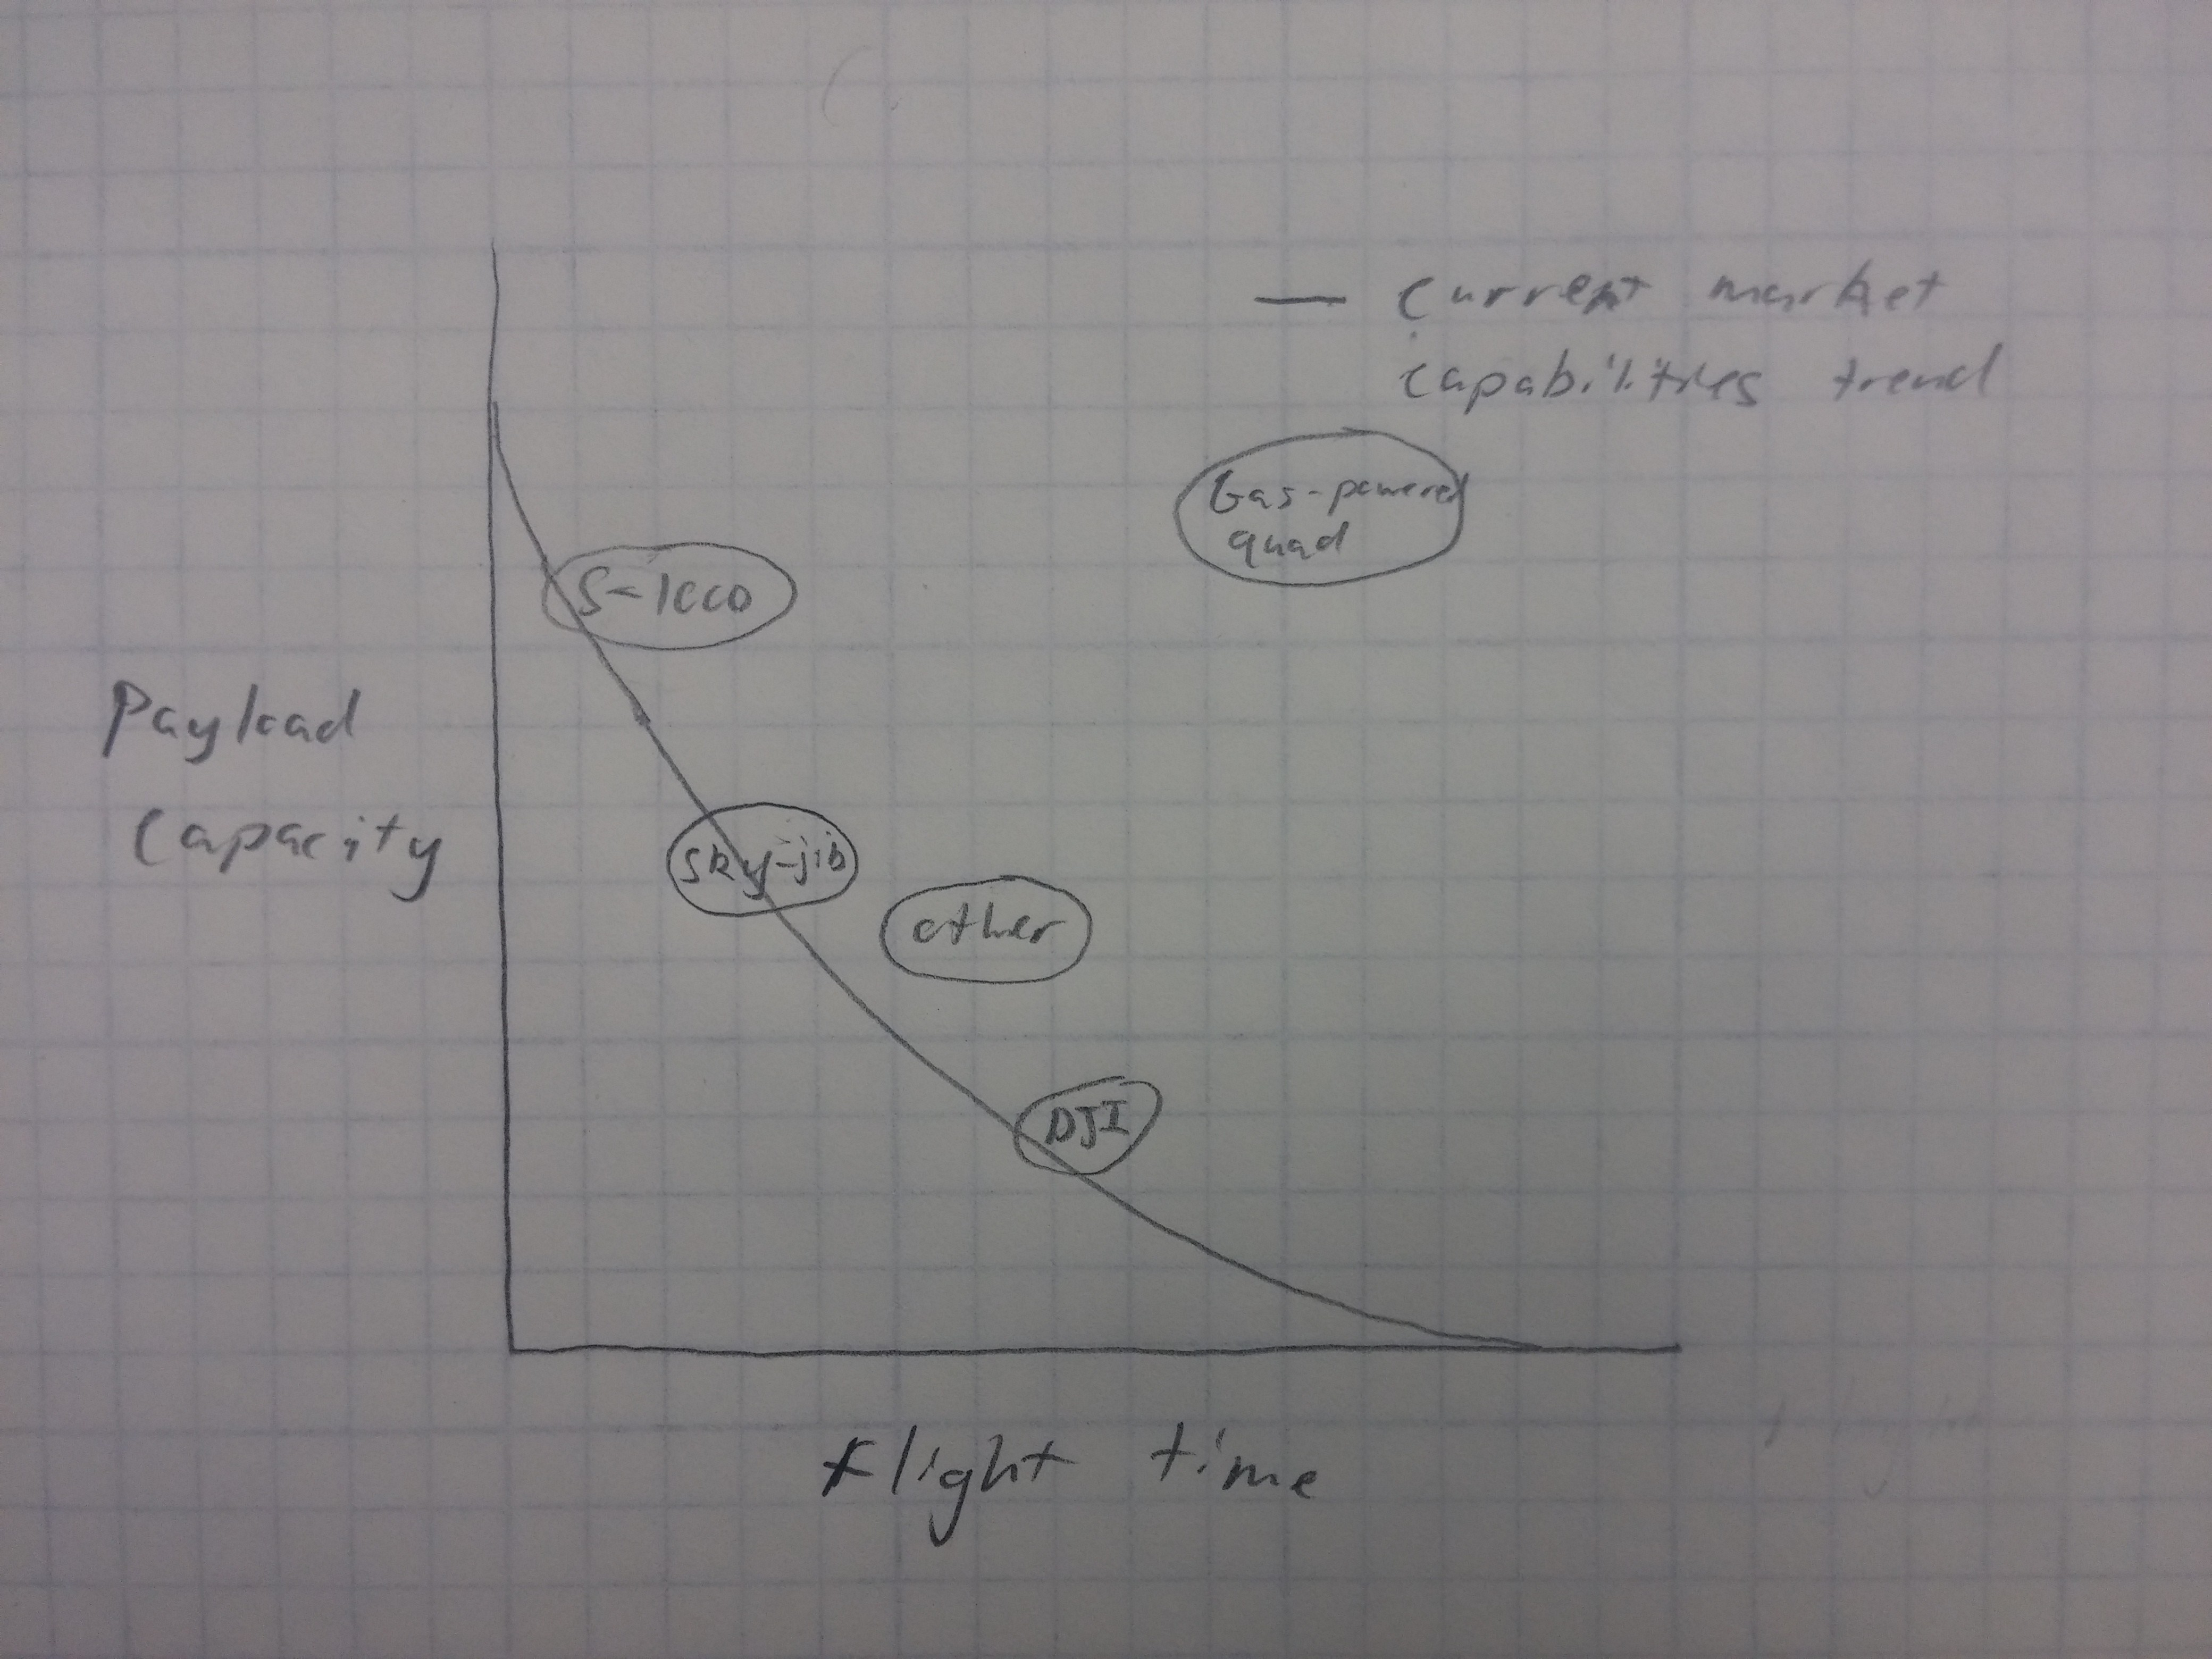
\includegraphics[width=.40\textwidth]{current_capabilities.jpg}
		\caption{\textit{Graphic showing current platforms and how our would be better.}}
		\label{current_cap}
	\end{center}
\end{figurehere}




	
%%%%%%%%%%%%%%%%%%%%%%%%%%%%%%%%%%%%%%%%%%%%%%%%%%%%%%%%%%%%%%%%%%%%%%%%%%%%%%%%%%
\section{METHODS}
analysis models

Empirical engine models
aerodynamic models
Simplifications - we are stupid

\section{OPTIMIZATION}
Setup the formal optimization problems

What optimizers, setup, comparing matlab and python. 
figure of Pareto fronts...

constraint sensitivity - aerodynamics, engine efficiencies...


%%%%%%%%%%%%%%%%%%%%%%%%%%%%%%%%%%%%%%%%%%%%%%%%%%%%%%%%%%%%%%%%%%%%%%%%%%%%%%%%%%

\section{CONCLUSION}

lots of really good conclusions

%%%%%%%%%%%%%%%%%%%%%%%%%%%%%%%%%%%%%%%%%%%%%%%%%%%%%%%%%%%%%%%%%%%%%%%%%%%%%%%%
% \section*{APPENDIX}

% Appendixes should appear before the acknowledgment.

% \section*{ACKNOWLEDGMENT}

% Important people/organizations who made it possible


%%%%%%%%%%%%%%%%%%%%%%%%%%%%%%%%%%%%%%%%%%%%%%%%%%%%%%%%%%%%%%%%%%%%%%%%%%%%%%%%

\bibliography{./library}
\bibliographystyle{ieeetr}



\end{document}


%%%%%%%%%%%%%%%%%%%%%%%%%%%%%%%%%%%%%%%%%%%%%%%%%%%%%%%%%%%%%%%%%%%%%%%%%%%%%

% SAVED STUFF






%new document




